\documentclass[10pt,a4paper]{article}
\usepackage[utf8]{inputenc}\usepackage[T1]{fontenc}\usepackage[german]{babel}
\usepackage{graphicx,float,booktabs,amsmath,siunitx,xcolor}
\usepackage[margin=2.2cm]{geometry}\usepackage[hidelinks]{hyperref}
\sisetup{output-decimal-marker={,}}
\hypersetup{pdfauthor={Thomas Schmiegelt},pdftitle={Kompakter Stellarator für 1 GW}}
\title{\textbf{Vom Stromnetz zur Spule: Auslegung eines kompakten\\Stellarators für 1\,GW elektrisch}\\[2pt]\large Version 0.3}
\author{Thomas Schmiegelt \textbar{} Hobbyprojekt \texttt{stellarator-design}}
\date{24.10.2026}
\begin{document}\maketitle

\noindent\fcolorbox{gray}{gray!8}{\parbox{0.96\linewidth}{\textbf{Hobbyprojekt, aus Neugier entstanden.}
Keine Verbindung zu einem Forschungsinstitut oder Unternehmen, nicht begutachtet. Alle Ergebnisse
sind Abschätzungen mit vereinfachten Modellen (0-D-Leistungsbilanz, Vakuumfeld, lineare Elastizität)
und können Fehler enthalten. Keine Auslegung einer realen Anlage.}}

\begin{abstract}
Die Frage wird vom Ziel her gestellt: Ein Kraftwerk soll \SI{1000}{MW} ins Netz liefern. Daraus folgt die
Fusionsleistung (\SI{3\,053}{MW}), daraus über Grenzen für Wandlast, Plasmadruck,
Dichte, Einschluss und Supraleiter die Größe $R_0$ und das Magnetfeld $B_0$. Eine optimierte,
quasi-axisymmetrische Plasmaform (DESC) wird mit Spulen (simsopt) erzeugt und unabhängig geprüft
(Feldlinien, Spulenfeld, Spalt, Kräfte). Eine Stützschale wird mit ElmerFEM in einem gekoppelten
Lauf (Magnetfeld $\to$ Lorentzkraft $\to$ Spannung) berechnet.
Ergebnis: Mit Seitenverhältnis $A=4{,}5$ reichen etwa $R_0\approx\SI{10,4}{m}$
(HTS) bzw. \SI{12,4}{m} (Nb$_3$Sn). Kritisch sind die Kräfte: über
\SI{1000}{MN} je Spule. Die Stützschale der Variante $A=6$ wiegt \SI{51}{kt} Stahl;
99\,\% der Schale liegen unter \SI{587}{MPa} (zulässig \SI{667}{MPa}),
örtliche Spitzen darüber.
\end{abstract}

\begin{figure}[H]\centering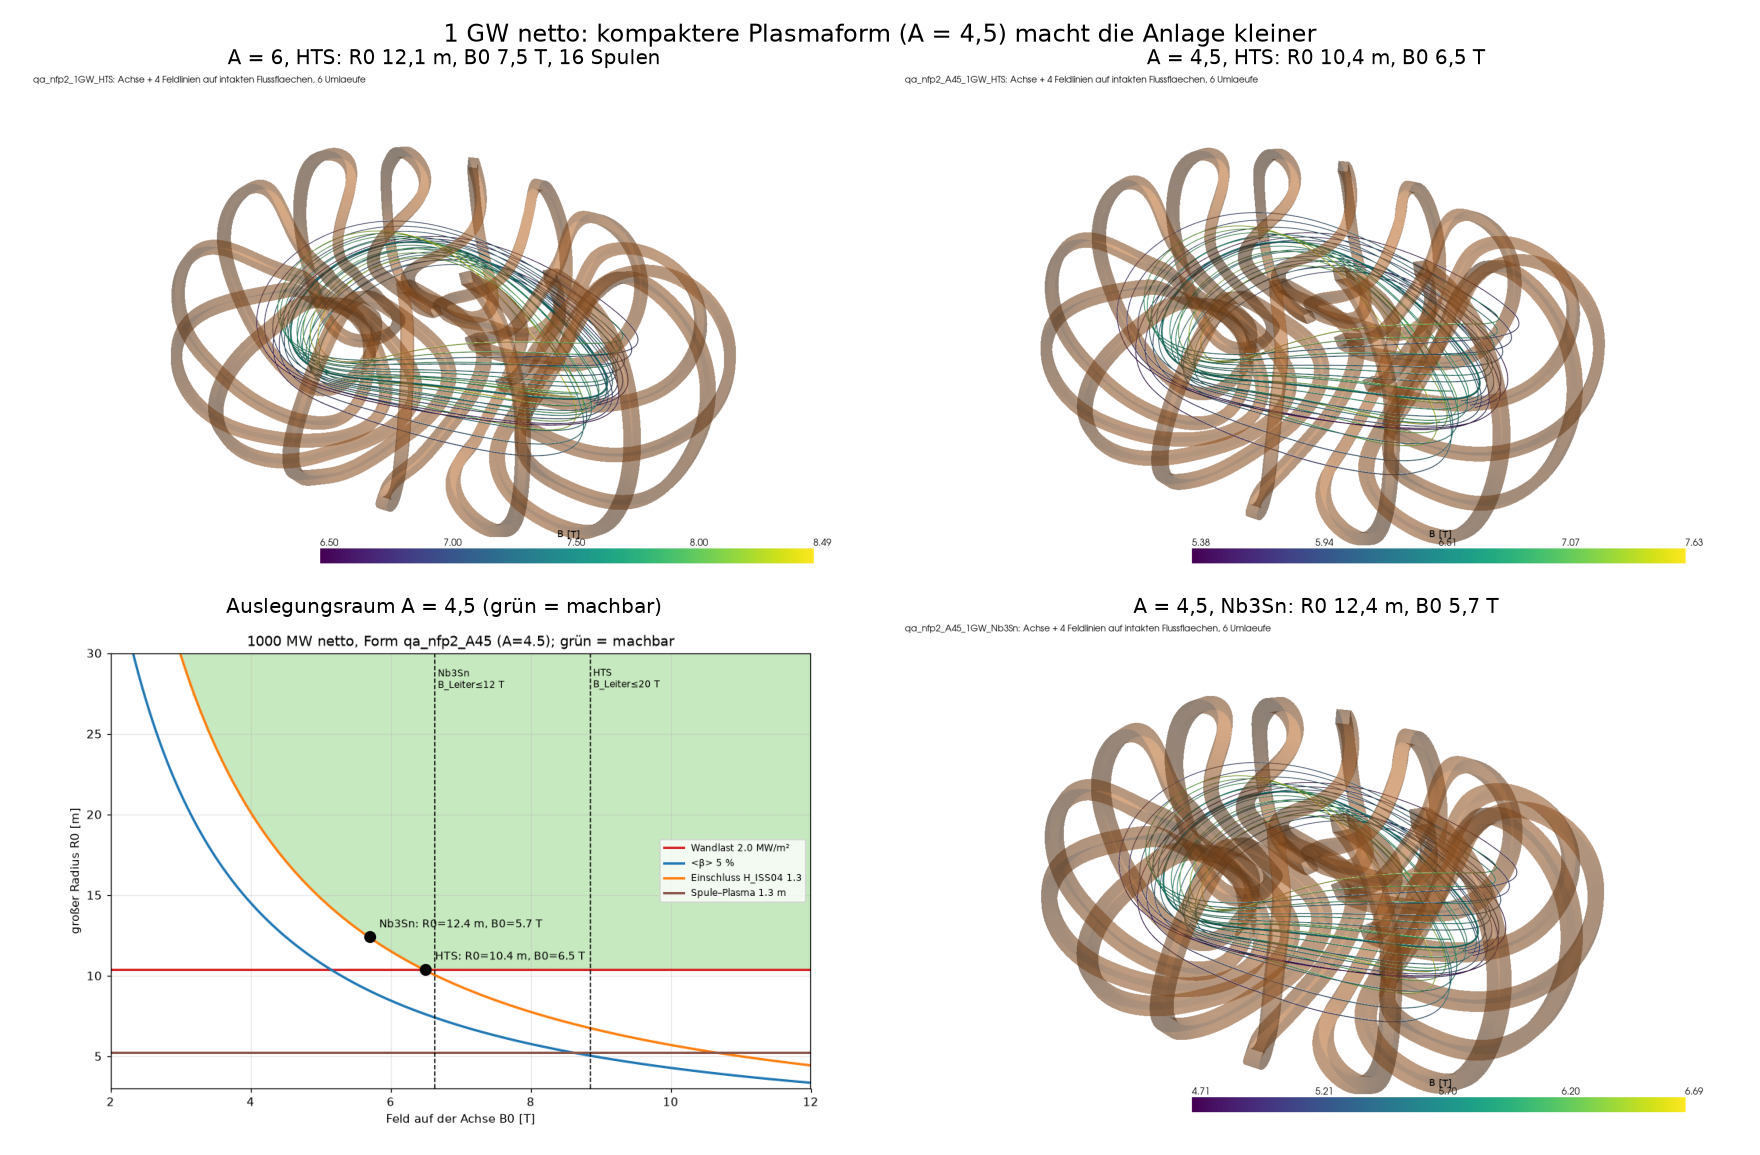
\includegraphics[width=1.0\linewidth]{bilder/uebersicht.png}\caption{Übersicht: kompaktere Plasmaform macht die Anlage kleiner (Feldlinien gefärbt nach $|B|$, Spulen braun). Die 3D-Bilder sind formatfüllend und nicht maßstäblich zueinander.}\end{figure}


\section{Die Kette vom Netz zum Plasma}
\begin{itemize}
\item \textbf{Plasma:} D-T-Fusion, je Reaktion \SI{17,6}{MeV}: \SI{80}{\%} trägt ein Neutron (\SI{14}{MeV}),
  \SI{20}{\%} ein Alpha-Teilchen. Die Alphas bleiben im Magnetfeld gefangen und heizen das Plasma
  (\SI{611}{MW}).
\item \textbf{Blanket:} Die Neutronen (\SI{2\,442}{MW}) durchdringen das Feld, werden im
  Blanket abgebremst (Energievervielfachung 1,15) und erbrüten Tritium aus Lithium.
\item \textbf{Kraftwerk:} Wärme \SI{3\,419}{MW}, Wirkungsgrad 0,35 $\to$
  brutto \SI{1\,197}{MW}, Eigenbedarf \SI{197}{MW}
  (Pumpen, Kälte, Anlage) $\to$ netto \SI{1\,000}{MW}.
\item \textbf{Magnetfeld:} hält nur geladene Teilchen. Es ist ein „Käfig“ für das \SI{150}{Mio.}\,°C heiße
  Plasma, durchlässig für Neutronen. Die verdrillten Spulen erzeugen geschlossene, geschachtelte
  Flussflächen ohne Plasmastrom (Dauerbetrieb).
\end{itemize}

\section{Methode}
\begin{description}
\item[Stufe 0 -- Leistungsbilanz] Raster über $(R_0, B_0, T_0)$; Fusionsleistung nach Bosch-Hale mit
  Parabelprofilen; Grenzen: Neutronen-Wandlast $\le$ \SI{2,0}{MW/m^2},
  $\langle\beta\rangle\le$ 5\,\%, Dichte $\le$ 1,5$\times$Sudo-Grenze,
  nötiger Einschluss $\le$ 1,3$\times$ISS04, Feld am Leiter (HTS \SI{20}{T}, Nb$_3$Sn \SI{12}{T}),
  Spule--Plasma $\ge$ \SI{1,3}{m}, Spalt zwischen Wickelpaketen $\ge$ \SI{0,2}{m}.
  Faktor Feld am Leiter / $B_0$ und Spaltmodell werden aus Stufe 3 iteriert.
\item[Stufe 1 -- Plasmaform] DESC, Vakuumgleichgewicht, Ziele Quasisymmetrie (QA), Seitenverhältnis, $\iota=0{,}42$, $n_\mathrm{fp}=2$.
\item[Stufe 2 -- Spulen] simsopt, 16 Spulen (4 Basisspulen und Symmetrie), $B\cdot n\to 0$ mit Strafen für Länge, Abstände, Krümmung.
\item[Stufe 3 -- Prüfung] eigene Biot-Savart-Rechnung, Feldlinien, $\iota$, Feld an der Wickeloberfläche, Kräfte, Spaltprüfung.
\item[Struktur] ElmerFEM: CoilSolver, WhitneyAV (Magnetostatik), Lorentzkraft $\vec J\times\vec B$ als Volumenlast im
  StressSolver; Stützschale aus Stahl (316LN, zulässig \SI{667}{MPa}) mit eingebetteten Wickelpaketen.
\end{description}

\section{Plasmaform und Spulen}
\begin{table}[H]\centering\begin{tabular}{lccccc}\toprule
Form & QS-Fehler [$10^{-5}$] & $\iota$ Achse & $\iota$ Rand & $|B\cdot n|/|B|$ Mittel [\%] & max [\%]\\\midrule
A = 6 & 1,3 & 0,423 & 0,415 & 0,11 & 0,40 \\
A = 4,5 & 2,4 & 0,425 & 0,412 & 0,27 & 0,96 \\
\bottomrule\end{tabular}
\caption{Stufe 1 und 2. Referenz DESC \emph{precise QA}: QS-Fehler $5{,}8\cdot10^{-5}$.}\end{table}
\begin{figure}[H]\centering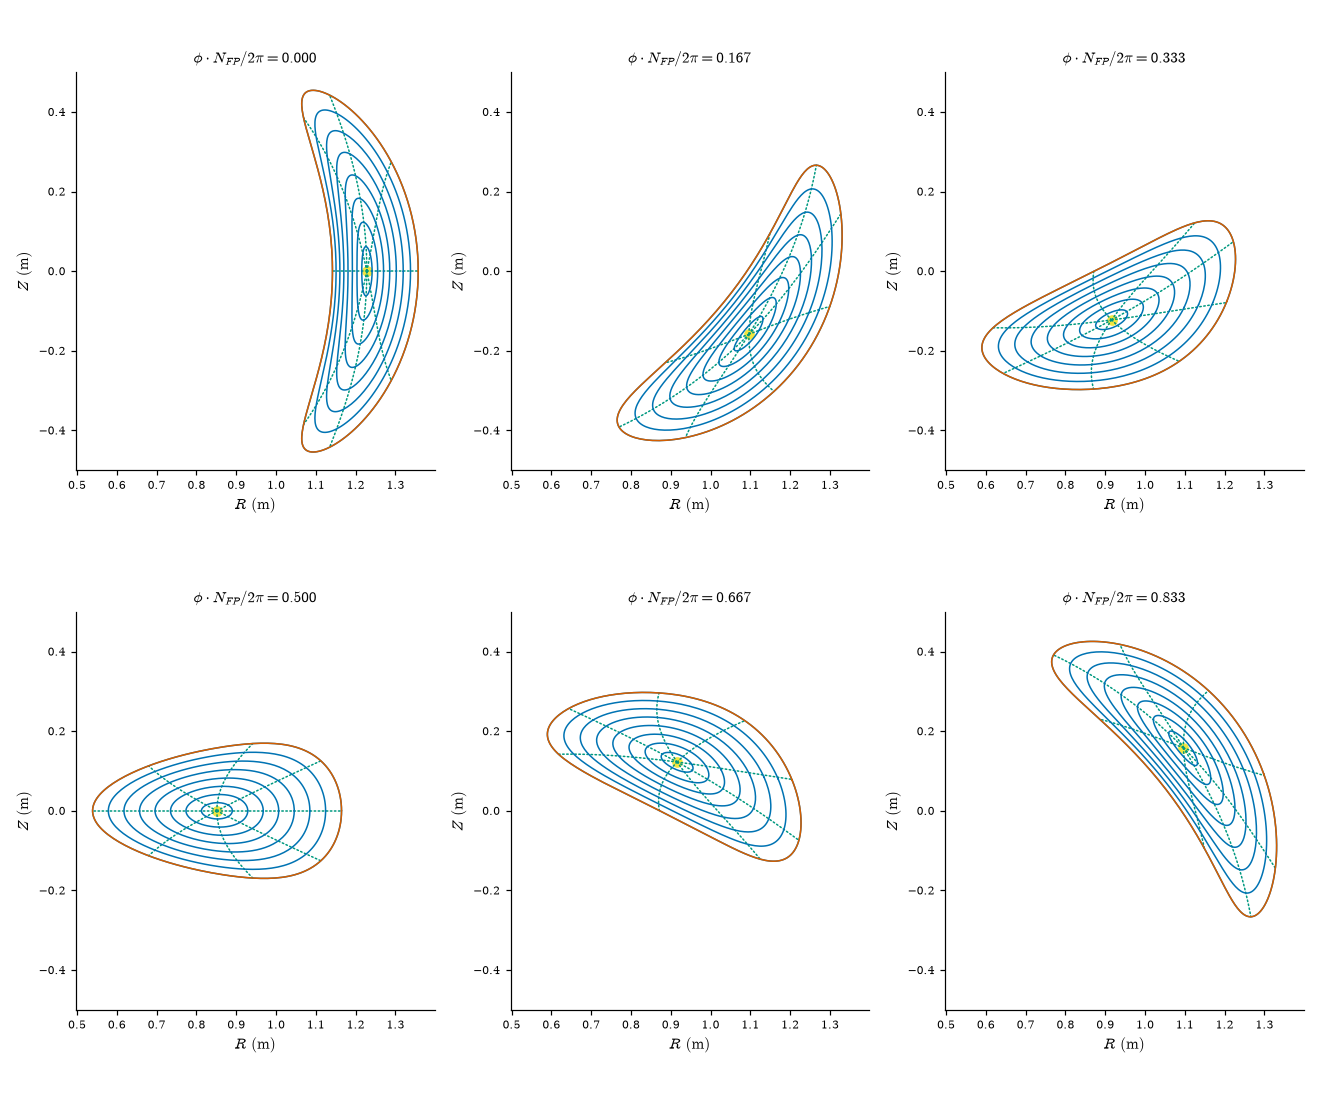
\includegraphics[width=0.55\linewidth]{bilder/A45_flaechen.png}\caption{Flussflächen der kompakten Form $A=4{,}5$ (DESC).}\end{figure}


\section{Auslegung auf 1\,GW und Prüfung in voller Größe}
\begin{table}[H]\centering\small\begin{tabular}{llcccccccc}\toprule
Form & Leiter & $R_0$ [m] & $a$ [m] & $B_0$ [T] & $B_\mathrm{Leiter}$ [T] & $I$ [MA] & Paket [m] & Spalt [m] & $F_\mathrm{max}$ [MN]\\\midrule
A = 6 & HTS & 12,1 & 2,0 & 7,50 & 17,7 & 31,0 & 0,88 & 0,58 & 2\,196 \\
A = 6 & Nb$_3$Sn & 22,2 & 3,7 & 4,80 & 11,6 & 36,4 & 1,56 & 1,13 & 3\,028 \\
A = 4,5 & HTS & 10,4 & 2,3 & 6,50 & 14,7 & 22,8 & 0,76 & 0,55 & 1\,196 \\
A = 4,5 & Nb$_3$Sn & 12,4 & 2,8 & 5,70 & 10,9 & 23,8 & 1,26 & 0,19 & 1\,307 \\
\bottomrule\end{tabular}
\caption{Auslegung (Stufe 0) und Prüfung (Stufe 3): Feld am Leiter, Strom je Spule, Spalt und Netto-Kraft aus der Biot-Savart-Rechnung in voller Größe.}\end{table}
\begin{figure}[H]\centering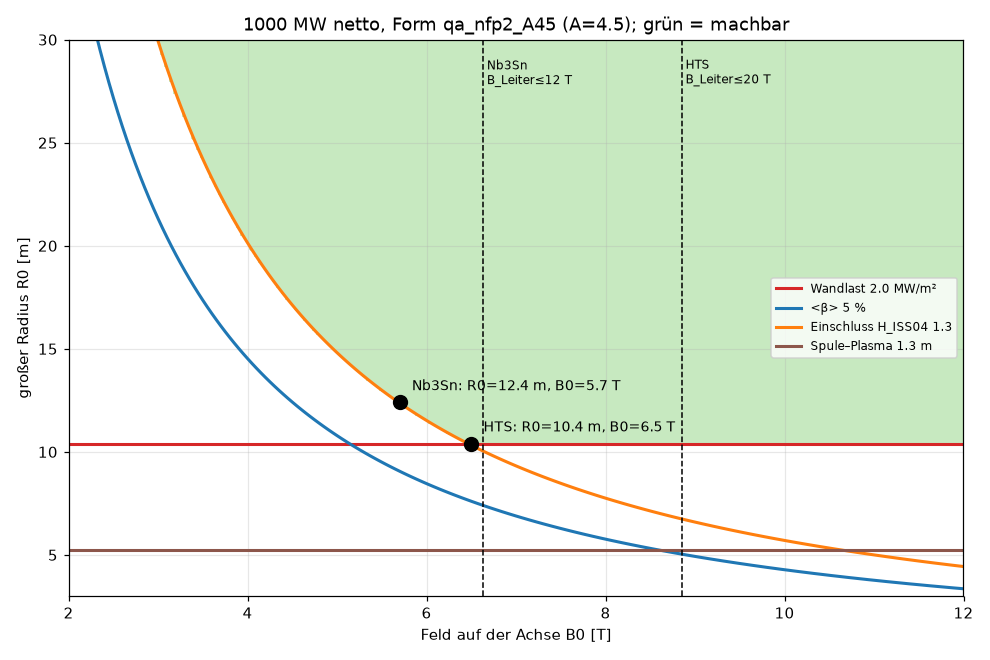
\includegraphics[width=0.75\linewidth]{bilder/A45_bilanz.png}\caption{Auslegungsraum für $A=4{,}5$: grün machbar, Linien = Grenzen.}\end{figure}

\begin{figure}[H]\centering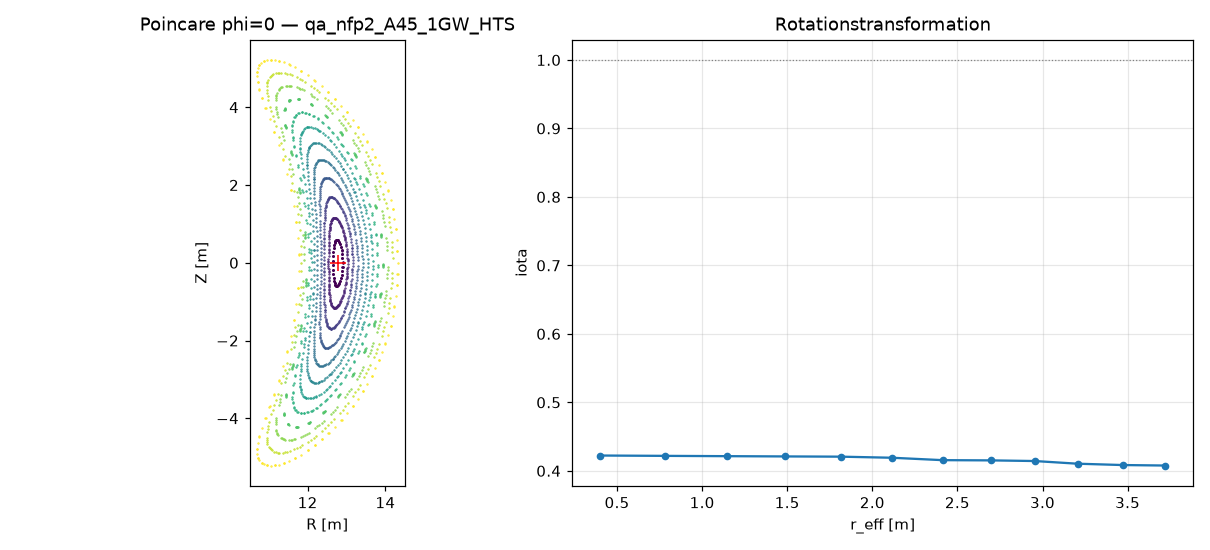
\includegraphics[width=0.8\linewidth]{bilder/A45_HTS_poincare.png}\caption{Poincaré-Schnitt und $\iota$-Profil der HTS-Auslegung $A=4{,}5$: alle Flussflächen intakt.}\end{figure}


\section{Stützstruktur (ElmerFEM)}
Die Lorentzkraft je Spule aus Elmer ($\int \vec J\times\vec B\,dV$) stimmt mit Biot-Savart überein: größte Spule 2\,259\,MN (Elmer) gegen 2\,196\,MN (Biot-Savart), Abweichung 2,9\,\%.
\begin{table}[H]\centering\small\begin{tabular}{lccccccc}\toprule
Form (HTS) & Dicke [m] & Masse [kt] & $\sigma_\mathrm{v}$ Mittel & 99\,\% unter & Spitze & Paket 99\,\% & $u_\mathrm{max}$ [mm]\\
 & & & [MPa] & [MPa] & [MPa] & [MPa] & \\\midrule
A = 6 & 1,48 & 50,7 & 187 & 587 & 1\,013 & 413 & 36 \\
A = 4,5 & \multicolumn{7}{l}{noch nicht gerechnet} \\
\bottomrule\end{tabular}
\caption{Von-Mises-Spannung in Schale und Wickelpaketen. Zulässig für 316LN bei \SI{4}{K}: \SI{667}{MPa}.}\end{table}
\begin{table}[H]\centering\small\begin{tabular}{lccccc}\toprule
Netz ($A=6$) & Tetraeder [Mio.] & Schale 99\,\% [MPa] & Schale Spitze [MPa] & Paket 99\,\% [MPa] & $u_\mathrm{max}$ [mm]\\\midrule
grob & 0,69 & 588 & 831 & 398 & 34 \\
mittel & 1,45 & 587 & 1\,013 & 413 & 36 \\
\bottomrule\end{tabular}
\caption{Netzstudie: die 99-\%-Werte sind konvergiert, die Spitzen wachsen (Spannungssingularität an den Paketecken).}\end{table}
\par\textit{(Bild A45 HTS struktur noch nicht erzeugt)}\par

\begin{figure}[H]\centering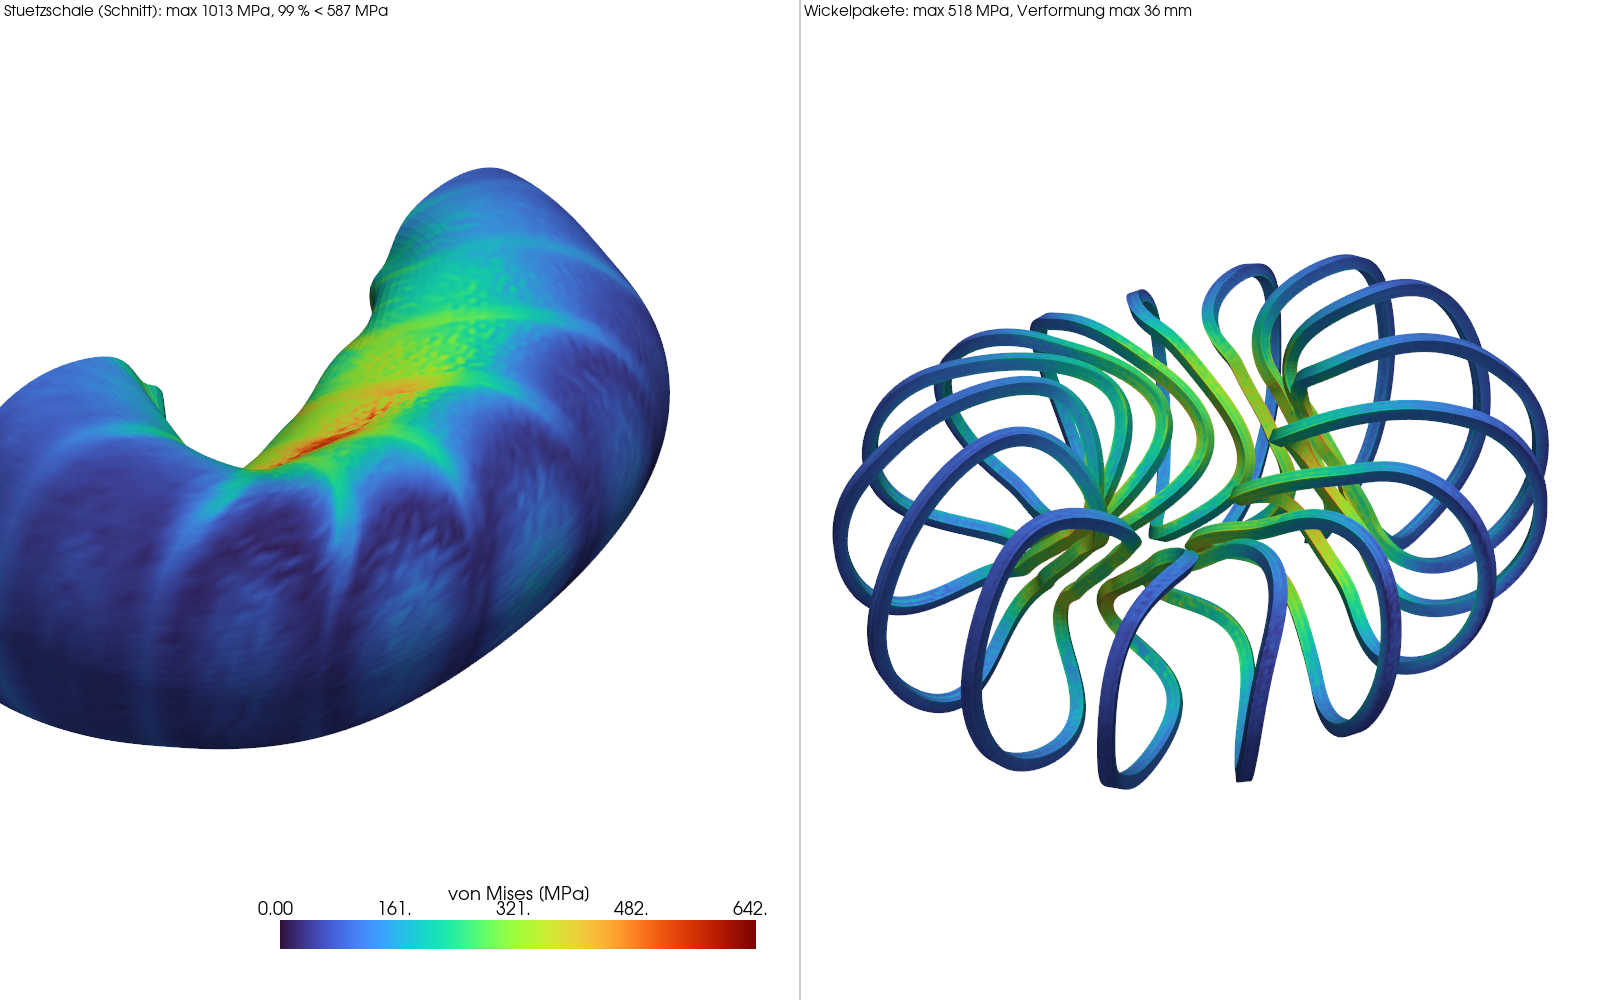
\includegraphics[width=1.0\linewidth]{bilder/A6_HTS_struktur.png}\caption{Von-Mises-Spannung, $A=6$ mit HTS.}\end{figure}


\section{Validierung}
W7-X mit realen Spulen: \SI{13,48}{kA} je Windung für
$\langle B\rangle_\mathrm{Achse}=\SI{2,5}{T}$, Spalt der Wickelpakete \SI{68}{mm}.
ElmerFEM gegen Biot-Savart mit allen 70 Spulen: Median-Abweichung auf der Achse 0,24\,\%.

\section{Erkenntnisse}
\begin{enumerate}
\item Der Einschluss (ISS04) bestimmt die Größe, bei HTS zusätzlich die Wandlast. Ein kleineres Seitenverhältnis
  verkleinert die Anlage deutlich; bei $A=4{,}5$ sind HTS und Nb$_3$Sn fast gleich groß.
\item Das Feld am Leiter ist kein fester Vielfacher von $B_0$: eng stehende Spulen ergaben $3{,}5\times B_0$,
  besser verteilte $1{,}8$--$2{,}4\times B_0$. Bei Nb$_3$Sn dominiert sonst das Eigenfeld des Wickelpakets
  (Stromdichte auf \SI{15}{A/mm^2} gesenkt).
\item Der Spulenstrom folgt aus dem Durchflutungsgesetz ($I\approx2\pi R_0B_0/\mu_0N$), unabhängig von der Spulenlage.
\item Die Spaltprüfung fand bei Nb$_3$Sn eine Durchdringung der Wickelpakete; der Spalt ist jetzt Teil von Stufe 0.
\item Kräfte von über \SI{1000}{MN} je Spule (W7-X: \SI{2}{MN}) machen die Stützstruktur zum Hauptproblem.
\end{enumerate}

\section{Grenzen und nächste Schritte}
\begin{itemize}
\item 0-D-Bilanz ($\pm30\,\%$): ohne Divertor-Wärmelast, Zyklotronstrahlung, Neutronik des Blankets.
\item Geometrie der Stützschale für allgemeine Spulenformen noch nicht robust: Flächen durch die
  Spulenkurven falten sich auf der Torus-Innenseite, die Vernetzung hängt bei dünnen Spalten.
  Für $A=4{,}5$ fehlt deshalb noch die Strukturrechnung.
\item Stützschale v1 ohne Öffnungen für Wartung und Heizung; Wickelpakete noch nicht an der Schalennormalen ausgerichtet
  (daher dicke Schale); Spannungsspitzen an Ecken $\to$ Ausrundungen, örtliche Verstärkung auf der Torus-Innenseite.
\item Zulässige Querdruckspannung der HTS-Bänder prüfen (Wickelpaket-Spannungen mehrere \SI{100}{MPa}).
\item Gewichtung Masse gegen Spannung: Schalendicke optimieren (Studien-Runner).
\end{itemize}

\begin{thebibliography}{9}\small
\bibitem{desc} D. Dudt, D. Panici, E. Kolemen: DESC stellarator equilibrium and optimization code, \url{https://github.com/PlasmaControl/DESC}.
\bibitem{simsopt} M. Landreman et al.: SIMSOPT, J. Open Source Softw. 6 (2021) 3525.
\bibitem{elmer} ElmerFEM, CSC -- IT Center for Science, \url{https://www.elmerfem.org}.
\bibitem{bh} H.-S. Bosch, G. M. Hale: Improved formulas for fusion cross-sections and thermal reactivities, Nucl. Fusion 32 (1992) 611.
\bibitem{iss04} H. Yamada et al.: Characterization of energy confinement in net-current free plasmas (ISS04), Nucl. Fusion 45 (2005) 1684.
\bibitem{sudo} S. Sudo et al.: Scalings of energy confinement and density limit in stellarator/heliotron devices, Nucl. Fusion 30 (1990) 11.
\bibitem{gmsh} C. Geuzaine, J.-F. Remacle: Gmsh, Int. J. Numer. Meth. Eng. 79 (2009) 1309.
\end{thebibliography}
\end{document}
